\documentclass[conference]{IEEEtran}
\IEEEoverridecommandlockouts
\usepackage{cite}
\usepackage{amsmath,amssymb,amsfonts}
\usepackage{graphicx}
\usepackage{booktabs}
\usepackage{textcomp}
\usepackage{xcolor}
\usepackage{tikz}
\usetikzlibrary{positioning,arrows.meta,fit,backgrounds}
\usepackage[hidelinks]{hyperref}
% auto-generated by make_tex_numbers.py -- do not edit
\newcommand{\Ntrials}{288}
\newcommand{\Nch}{59}
\newcommand{\Fs}{150.15}
\newcommand{\Dur}{4.6}
\newcommand{\NLA}{72}
\newcommand{\NRA}{73}
\newcommand{\NLV}{73}
\newcommand{\NRV}{70}
\newcommand{\ANlat}{100}
\newcommand{\ANamp}{-3.1}
\newcommand{\APlat}{166}
\newcommand{\APamp}{2.3}
\newcommand{\VPlat}{100}
\newcommand{\VPamp}{2.0}
\newcommand{\VNlat}{173}
\newcommand{\VNamp}{-3.5}
\newcommand{\ChanceMod}{50.3}
\newcommand{\AccModX}{98.2}
\newcommand{\SdModX}{0.2}
\newcommand{\KapModX}{0.96}
\newcommand{\AucModX}{0.999}
\newcommand{\AccModC}{92.2}
\newcommand{\SdModC}{1.2}
\newcommand{\KapModC}{0.84}
\newcommand{\AucModC}{0.958}
\newcommand{\AccModT}{80.1}
\newcommand{\SdModT}{1.1}
\newcommand{\KapModT}{0.60}
\newcommand{\AucModT}{0.856}
\newcommand{\ChanceFour}{25.3}
\newcommand{\AccFourX}{83.9}
\newcommand{\SdFourX}{2.0}
\newcommand{\KapFourX}{0.78}
\newcommand{\AccFourC}{71.2}
\newcommand{\SdFourC}{1.4}
\newcommand{\KapFourC}{0.62}
\newcommand{\AccFourT}{53.6}
\newcommand{\SdFourT}{1.5}
\newcommand{\KapFourT}{0.38}
\newcommand{\ChanceAudLat}{50.3}
\newcommand{\AccAudLatX}{71.2}
\newcommand{\SdAudLatX}{2.8}
\newcommand{\KapAudLatX}{0.42}
\newcommand{\AucAudLatX}{0.779}
\newcommand{\AccAudLatC}{58.6}
\newcommand{\SdAudLatC}{2.5}
\newcommand{\KapAudLatC}{0.17}
\newcommand{\AucAudLatC}{0.636}
\newcommand{\AccAudLatT}{53.0}
\newcommand{\SdAudLatT}{3.3}
\newcommand{\KapAudLatT}{0.06}
\newcommand{\AucAudLatT}{0.551}
\newcommand{\ChanceVisLat}{51.0}
\newcommand{\AccVisLatX}{97.6}
\newcommand{\SdVisLatX}{0.6}
\newcommand{\KapVisLatX}{0.95}
\newcommand{\AucVisLatX}{0.995}
\newcommand{\AccVisLatC}{93.1}
\newcommand{\SdVisLatC}{1.4}
\newcommand{\KapVisLatC}{0.86}
\newcommand{\AucVisLatC}{0.975}
\newcommand{\AccVisLatT}{75.8}
\newcommand{\SdVisLatT}{3.8}
\newcommand{\KapVisLatT}{0.52}
\newcommand{\AucVisLatT}{0.825}
\newcommand{\PermP}{0.005}
\newcommand{\Nperm}{200}
\newcommand{\ChronoMod}{97.9}
\newcommand{\ChronoFour}{80.6}
\newcommand{\Ncal}{144}
\newcommand{\Ntest}{144}
\newcommand{\LCfirstN}{10}
\newcommand{\LCfirst}{67.9}
\newcommand{\LClastN}{200}
\newcommand{\LClast}{98.1}
\newcommand{\DetANkOne}{35}
\newcommand{\DetANkTwo}{45}
\newcommand{\DetANkFour}{49}
\newcommand{\DetANkEight}{71}
\newcommand{\DetANkOneSix}{84}
\newcommand{\DetANkThreeTwo}{98}
\newcommand{\KNinetyAN}{32}
\newcommand{\FAmaxAN}{19}
\newcommand{\FAkmaxAN}{15}
\newcommand{\DetkmaxAN}{98}
\newcommand{\Kmax}{32}
\newcommand{\DetkoneAN}{35}
\newcommand{\DetVPkOne}{15}
\newcommand{\DetVPkTwo}{22}
\newcommand{\DetVPkFour}{22}
\newcommand{\DetVPkEight}{33}
\newcommand{\DetVPkOneSix}{40}
\newcommand{\DetVPkThreeTwo}{46}
\newcommand{\KNinetyVP}{--}
\newcommand{\FAmaxVP}{27}
\newcommand{\FAkmaxVP}{26}
\newcommand{\DetkmaxVP}{46}
\newcommand{\DetkoneVP}{15}
\newcommand{\KavgAccA}{98.1}
\newcommand{\KavgKA}{1}
\newcommand{\KavgAccB}{99.7}
\newcommand{\KavgKB}{2}
\newcommand{\KavgAccC}{100.0}
\newcommand{\KavgKC}{3}
\newcommand{\KavgAccD}{100.0}
\newcommand{\KavgKD}{5}
\newcommand{\Decim}{4}
\newcommand{\AudConfShare}{89}
\newcommand{\ClusterFC}{021, 031, 030, 032, 013}
\newcommand{\ClusterO}{060, 058, 059, 057, 056}
\newcommand{\RosExcess}{15.4}
\newcommand{\RosExcessSd}{5.6}
\newcommand{\RosExcessP}{22.5}
\newcommand{\RosTotal}{508.7}
\newcommand{\RosProc}{6.50}
\newcommand{\RosAgree}{100}
\newcommand{\RosNdec}{1728}
\newcommand{\RosNmark}{1728}
\newcommand{\RosMaxExcess}{75.4}
\newcommand{\RosCpuDet}{8.5}
\newcommand{\RosCpuAll}{44.9}
\newcommand{\RosRss}{489}
\newcommand{\RosFastExMin}{3.8}
\newcommand{\RosFastExMax}{4.3}
\newcommand{\RosFastProc}{1.7}
\newcommand{\RosExTen}{11.6}
\newcommand{\RosExForty}{23.5}
\newcommand{\RosCpuFast}{92}

\newcommand{\ISImed}{699}
\newcommand{\ISImin}{593}
\newcommand{\ISImax}{1112}
\newcommand{\RecallLA}{68.2}
\newcommand{\RecallRA}{72.6}
\newcommand{\RecallLV}{98.5}
\newcommand{\RecallRV}{96.4}
\newcommand{\Nfilt}{12}
\newcommand{\Nfeat}{276}
\newcommand{\CpuStreamer}{25.3}
\newcommand{\CpuDet}{8.5}
\newcommand{\CpuStreamerFast}{49.8}

\newcommand{\RieMod}{97.8}
\newcommand{\RiePMod}{0.58}
\newcommand{\RieFour}{81.0}
\newcommand{\RiePFour}{0.31}
\newcommand{\RieAudLat}{67.0}
\newcommand{\RiePAudLat}{0.49}
\newcommand{\RieVisLat}{97.8}
\newcommand{\RiePVisLat}{0.85}
\newcommand{\PClusterMax}{0.05}
\newcommand{\PreMin}{50.2}
\newcommand{\PreMax}{50.8}
\newcommand{\PreFourMin}{25.1}
\newcommand{\PreFourMax}{29.3}
\newcommand{\OffCycleN}{16}
\newcommand{\OffCycleMod}{99.4}
\newcommand{\OffCycleFour}{76.9}
\newcommand{\CycleFrac}{94.4}
\newcommand{\PrevPred}{95.1}
\newcommand{\EogMod}{59.7}
\newcommand{\EogVis}{54.5}
\newcommand{\EogFour}{31.4}
\newcommand{\EogRegMod}{98.3}
\newcommand{\EogRegVis}{97.8}
\newcommand{\FrontMod}{97.6}
\newcommand{\FrontVis}{97.6}
\newcommand{\FrontAud}{66.7}
\newcommand{\FrontN}{20}
\newcommand{\PermThousandP}{0.001}
\newcommand{\PermNullMax}{60.4}
\newcommand{\GdTen}{18}
\newcommand{\GdFive}{30}
\newcommand{\ShiftN}{6.7}
\newcommand{\ShiftP}{13.3}
\newcommand{\ZpN}{93}
\newcommand{\ZpP}{87}
\newcommand{\FairNThirtyTwo}{98.7}
\newcommand{\FairNFa}{7.7}
\newcommand{\FairNSixteen}{80.0}
\newcommand{\FairPThirtyTwo}{30.7}
\newcommand{\FairPFa}{10.0}
\newcommand{\RobotN}{288}
\newcommand{\RobotHeldN}{144}
\newcommand{\RobotAcc}{98.6}
\newcommand{\RobotErr}{2}
\newcommand{\RobotCmd}{1.23}
\newcommand{\RobotCmdP}{1.49}
\newcommand{\RobotOnset}{510}
\newcommand{\RobotOnsetSd}{5.7}
\newcommand{\RobotOnsetMax}{519}
\newcommand{\LastSample}{493}
\newcommand{\RobotExcess}{15.8}

\newcommand{\SpExcess}{13.2}
\newcommand{\SpExcessSd}{6.1}
\newcommand{\SpProc}{6.2}
\newcommand{\RrExcess}{15.6}
\newcommand{\RrExcessSd}{5.5}
\newcommand{\Overhead}{2.3}


\begin{document}

\title{A ROS~2 Pipeline for Real-Time Single-Trial Discrimination of Visual and Auditory Evoked Potentials from Multichannel EEG}

\author{\IEEEauthorblockN{Vinoth S}
\IEEEauthorblockA{\textit{Department of Biomedical Engineering} \\
\textit{Kalaignarkarunanidhi Institute of Technology (KIT)}\\
Coimbatore, Tamil Nadu, India}
}

\maketitle

\begin{abstract}
Visual (VEP) and auditory (AEP) evoked potentials are routine clinical and brain--computer interface markers, yet they are usually analysed offline after many trials have been averaged. We present an open Robot Operating System~2 (ROS~2) pipeline that discriminates VEPs and AEPs trial by trial in streaming multichannel electroencephalography (EEG). Four nodes perform amplifier emulation, causal filtering with common-average referencing, stimulus-locked epoching, and classification with xDAWN spatial filtering and shrinkage linear discriminant analysis (LDA); decisions are published as typed ROS~2 messages. On the public MNE sample recording (\Nch{} channels, \Ntrials{} lateralised tone and checkerboard trials), single trials were assigned to the correct modality with \AccModX\,\% accuracy (permutation $p=\PermThousandP$) and to one of four stimulus classes with \AccFourX\,\%. This matched a Riemannian tangent-space classifier and significantly exceeded fixed-channel LDA and template matching. Control analyses showed that the result is explained neither by the fixed stimulus order (pre-stimulus decoding at chance; \OffCycleMod\,\% on off-cycle trials) nor by eye movements (unchanged after EOG regression or removal of frontal channels). A classical 3-SD peak criterion needed 32-trial averages to detect the AEP N1 and failed for the VEP P1. Under ROS~2 on a desktop PC, every stimulus produced a decision \RosExcess\,ms (mean) after its epoch ended, identical to the offline output, and a turtlesim robot executed the intended action on \RobotAcc\,\% of held-out trials, \RobotCmd\,ms after each decision.
\end{abstract}

\begin{IEEEkeywords}
EEG, visual evoked potential, auditory evoked potential, ROS~2, xDAWN, single-trial classification, real-time signal processing, brain--computer interface
\end{IEEEkeywords}

\section{Introduction}
Evoked potentials (EPs) are the time-locked responses of the brain to sensory stimuli. The pattern-reversal or flash VEP, dominated by a positive occipital deflection near 100\,ms (P1/P100), is a standard test of the visual pathway~\cite{odom2016iscev}. The long-latency AEP, characterised by a fronto-central negativity near 100\,ms (N1) and a later positivity (P2), indexes auditory cortical processing; the N1 in particular has well-characterised cortical generators~\cite{naatanen1987n1}. Because EPs are only a few microvolts in amplitude and are buried in the ongoing EEG, the conventional practice is to average tens to hundreds of stimulus repetitions offline and then measure peak latency and amplitude by hand~\cite{picton2000guidelines}.

Single-trial analysis has changed this picture in BCI research. Spatial filtering combined with regularised linear classifiers can recover event-related potentials (ERPs) from individual epochs~\cite{blankertz2011tutorial,krusienski2006comparison,lotte2018review}, and the xDAWN algorithm enhances the evoked subspace by maximising the signal-to-signal-plus-noise ratio~\cite{rivet2009xdawn}. Hybrid BCIs combine more than one input signal~\cite{pfurtscheller2010hybrid}, and gaze-independent spellers have combined visual and auditory stimuli~\cite{an2014exploring}. A system that knows, trial by trial, \emph{which} sensory pathway responded is useful in several settings: objective screening of the visual versus auditory pathway, monitoring of stimulus delivery, and multimodal BCIs that route a user's intention to an assistive robot~\cite{wolpaw2002bci}.

Deploying such detectors on robots requires a software substrate that is real-time capable, distributed and interoperable. ROS~2 provides publish--subscribe communication over the Data Distribution Service (DDS) with configurable quality of service (QoS) and is now the de facto standard in robotics~\cite{macenski2022ros2,maruyama2016exploring}. EEG streaming has traditionally relied on the Lab Streaming Layer (LSL)~\cite{kothe2025lsl}. Beraldo~\emph{et al.} first coupled a BCI with ROS to drive a telepresence robot~\cite{beraldo2018bciros}, and ROS-Neuro generalised this into a neurorobotics framework for ROS~1~\cite{tonin2022rosneuro}. On the decoding side, Putze~\emph{et al.} discriminated visual from auditory perception with 97.8\,\% subject-dependent accuracy using hybrid EEG--fNIRS~\cite{putze2014hybrid}. Massaeli~\emph{et al.} distinguished auditory from visual processing tasks with 77.1\,\% accuracy at high demand~\cite{massaeli2023modality}. These studies classified multi-second task periods offline, however, not individual evoked responses in a streaming system. To our knowledge, no open ROS~2 pipeline has been reported for the trial-by-trial discrimination of VEPs and AEPs, nor has the equivalence between its streamed and offline results been quantified.

Our contributions are:
\begin{enumerate}
\item an open ROS~2 package (tested on Jazzy and Lyrical) with four nodes for streaming, causal preprocessing, epoching and single-trial VEP/AEP classification, and a typed decision message;
\item a single-trial evaluation on public EEG of modality, four-class and laterality discrimination against three baselines with corrected statistics, including controls for the stimulus order and for eye movements;
\item a comparison with the classical averaging-based peak criterion in terms of hit and false-alarm rates;
\item measured latency, middleware overhead, robustness to message loss and resource use under ROS~2, and a closed demonstration in which the decisions drive a simulated robot.
\end{enumerate}

\section{Materials and Methods}

\subsection{Dataset}
We used the publicly available MNE ``sample'' recording~\cite{gramfort2013mne}, acquired with a Neuromag Vectorview MEG/EEG system at the MGH/HMS/MIT Martinos Center. One healthy adult received monaural tone pips to the left or right ear (LA, RA) and checkerboard patterns in the left or right visual hemifield (LV, RV). According to the dataset documentation, stimuli were nominally 750\,ms apart, and the subject pressed a key with the right index finger whenever an occasional smiley face appeared at fixation~\cite{gramfort2013mne}. Checker size, contrast, tone frequency and intensity are not reported. The stimuli were not randomised: in the event log, 272 of the 287 transitions (94.8\,\%) follow the fixed cycle RA$\rightarrow$LV$\rightarrow$LA$\rightarrow$RV. The remaining 15 occur after pauses longer than 1\,s, in which other events (not analysed here) were presented. Auditory and visual stimuli therefore almost always alternate, a confound we test explicitly in Section~\ref{sec:ctl}. Simultaneous 60-channel EEG was recorded; after removing the channel marked bad, \Nch{} channels remain. We used the distributed version, which is low-pass filtered at 40\,Hz and decimated to \Fs\,Hz (\Dur\,min). There were \NLA, \NRA, \NLV{} and \NRV{} LA, RA, LV and RV trials, respectively (\Ntrials{} in total). Only the EEG channels were used; the magnetometer and gradiometer channels were discarded. Fig.~\ref{fig:paradigm} illustrates the four stimulus classes and the first 20\,s of the stimulus sequence reconstructed from the event log. Stimuli followed one another with a median inter-stimulus interval (ISI) of \ISImed\,ms (minimum \ISImin\,ms, 95th percentile \ISImax\,ms). The 600-ms analysis epoch therefore usually ends close to the onset of the next stimulus. A detector must cope with this overlap, because the late part of one response coincides with the baseline of the next.

\begin{figure}[t]
\centering
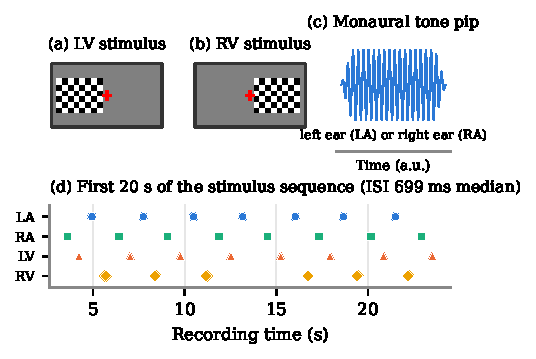
\includegraphics[width=\columnwidth]{fig_paradigm.pdf}
\caption{Stimulation paradigm. (a, b) Schematic of the hemifield checkerboard stimuli with central fixation cross (illustrative rendering, not a screen capture). (c) Schematic monaural tone pip. (d) Actual onsets of the four classes in the first 20\,s of the recording.}
\label{fig:paradigm}
\end{figure}

\subsection{ROS~2 Architecture}
Fig.~\ref{fig:arch} shows the four-node graph. All topics use reliable QoS with a keep-last history of depth 200.
\begin{itemize}
\item \texttt{eeg\_streamer} emulates an amplifier. It replays the recording in chunks of $L$ samples (default 20\,ms) at a configurable speed on \texttt{/eeg/raw} (\texttt{Float32MultiArray}; the field \texttt{data\_offset} carries the absolute index of the first sample). Stimulus markers are published on \texttt{/eeg/markers} as $[s_k, c_k, t_k]$: onset sample, event code, and the wall-clock time at which the onset sample was acquired.
\item \texttt{erp\_preprocessor} applies the causal filter and the common-average reference (Section~\ref{sec:pre}) and publishes \texttt{/eeg/filtered}.
\item \texttt{erp\_detector} stores filtered data in a ring buffer indexed by absolute sample number. When the post-stimulus window of a pending marker is complete, it extracts, classifies and publishes a JSON decision on \texttt{/erp/decision}. Gaps in \texttt{data\_offset} are detected, and any epoch that overlaps a gap is rejected.
\item \texttt{erp\_evaluator} logs decisions, accuracy and timing.
\end{itemize}
Because the streamer can be replaced by an LSL or vendor driver node, and a robot controller can subscribe to \texttt{/erp/decision}, the detector is independent of both the hardware and the application.

\begin{figure}[t]
\centering
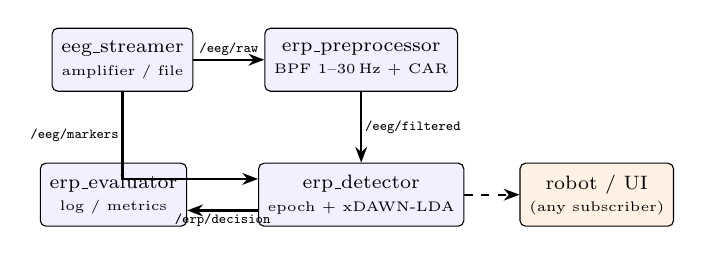
\begin{tikzpicture}[node distance=4mm and 5mm, font=\scriptsize,
  nd/.style={draw, rounded corners=2pt, fill=blue!6, minimum width=17mm, minimum height=8mm, align=center},
  tp/.style={font=\tiny\ttfamily, inner sep=1pt},
  ar/.style={-{Stealth[length=2mm]}, thick}]
\node[nd] (s) {eeg\_streamer\\\tiny amplifier / file};
\node[nd, right=9mm of s] (p) {erp\_preprocessor\\\tiny BPF 1--30\,Hz + CAR};
\node[nd, below=9mm of p] (d) {erp\_detector\\\tiny epoch + xDAWN-LDA};
\node[nd, left=9mm of d] (e) {erp\_evaluator\\\tiny log / metrics};
\node[nd, right=7mm of d, fill=orange!10] (r) {robot / UI\\\tiny (any subscriber)};
\draw[ar] (s) -- node[tp, above] {/eeg/raw} (p);
\draw[ar] (p) -- node[tp, right] {/eeg/filtered} (d);
\draw[ar] (s.south) |- node[tp, pos=0.25, left] {/eeg/markers} ([yshift=2mm]d.west);
\draw[ar] ([yshift=-2mm]d.west) -- node[tp, below] {/erp/decision} ([yshift=-2mm]e.east);
\draw[ar, dashed] (d) -- (r);
\end{tikzpicture}
\caption{ROS~2 computation graph of the proposed VEP/AEP pipeline.}
\label{fig:arch}
\end{figure}

\subsection{Causal Preprocessing}\label{sec:pre}
Each chunk $\mathbf{X}\in\mathbb{R}^{L\times C}$ is filtered by a fourth-order Butterworth band-pass (1--30\,Hz) implemented as second-order sections. The per-channel filter state $\mathbf{z}$ is carried from chunk to chunk, so the streamed output is sample-for-sample identical to filtering the whole recording at once. A common-average reference (CAR), $\tilde{x}_c[n]=x_c[n]-\frac{1}{C}\sum_{j}x_j[n]$, follows. A zero-phase filter is deliberately avoided because it is non-causal and would make the offline and online signals differ.

\subsection{Epoching}
For a marker at sample $s_k$, the epoch $\mathbf{E}_k\in\mathbb{R}^{C\times T}$ spans $[-100, 500]$\,ms and is corrected by subtracting the mean of the pre-stimulus interval. The decision cannot be issued before the epoch ends, so the window length sets a lower bound of 500\,ms on the marker-to-decision latency.

\subsection{xDAWN Spatial Filtering and Shrinkage LDA}
For each class $q$, let $\bar{\mathbf{E}}_q$ be the class-average epoch, $\mathbf{C}_q=\mathrm{cov}(\bar{\mathbf{E}}_q)$, and $\mathbf{C}_x$ the covariance of the concatenated single-trial epochs, regularised as $\mathbf{C}_x+\epsilon\,\frac{\mathrm{tr}(\mathbf{C}_x)}{C}\mathbf{I}$ with $\epsilon=10^{-3}$. The xDAWN filters~\cite{rivet2009xdawn} solve the generalised eigenproblem
\begin{equation}
\mathbf{C}_q\,\mathbf{w}=\lambda\,\mathbf{C}_x\,\mathbf{w},
\end{equation}
which maximises the ratio of evoked to total power. The $F=3$ leading eigenvectors of each class are stacked into $\mathbf{W}\in\mathbb{R}^{3Q\times C}$. The projected epoch $\mathbf{W}\mathbf{E}_k$ is low-pass filtered and decimated by \Decim{} (to about 37.5\,Hz), then vectorised into $\mathbf{f}_k$. Classification uses LDA,
\begin{equation}
\hat{y}_k=\arg\max_q\;\boldsymbol{\beta}_q^{\top}\mathbf{f}_k+b_q,\quad \boldsymbol{\beta}_q=\hat{\boldsymbol{\Sigma}}^{-1}\boldsymbol{\mu}_q,
\end{equation}
where $\hat{\boldsymbol{\Sigma}}=(1-\gamma)\mathbf{S}+\gamma\nu\mathbf{I}$ is the Ledoit--Wolf shrinkage estimate of the pooled covariance, with $\gamma$ chosen analytically~\cite{ledoit2004well,blankertz2011tutorial}. At run time the detector needs only $\mathbf{W}$, $\boldsymbol{\beta}_q$ and $b_q$, which are stored as a small NumPy file.

\paragraph*{Baselines} \emph{Cluster-LDA} applies the same shrinkage LDA to the decimated waveforms of two fixed clusters of five electrodes each: a fronto-central cluster just anterior to the vertex (EEG \ClusterFC) and an occipital cluster (EEG \ClusterO). Both clusters were chosen from the sensor geometry alone. \emph{Template} assigns each trial to the class whose spatio-temporal average template has the highest Pearson correlation with it. \emph{Riemann-TS} applies the Riemannian tangent-space approach~\cite{barachant2012riemann} to xDAWN-augmented covariance matrices (3 filters per class, Ledoit--Wolf estimates) and classifies them with logistic regression.

\subsection{Classical Detection by Averaging}
To connect the pipeline with clinical practice, we also detected the AEP N1 (fronto-central cluster, negative peak in 70--150\,ms) and the VEP P1 (occipital cluster, positive peak in 70--160\,ms) in averages of $k$ randomly drawn trials, $k\in\{1,2,4,\dots,32\}$. A component counted as present when its peak exceeded three times the noise standard deviation, estimated over the whole epoch from the $\pm$-reference of the same $k$ trials (alternate trials sign-inverted so that the evoked response cancels while the noise remains~\cite{picton2000guidelines}). False alarms were estimated by applying the same rule to an independent $\pm$-reference average. Each $k$ was resampled 300 times.

\subsection{Implementation Details}
All nodes use Python (\texttt{rclpy}, NumPy, SciPy) in one \texttt{ament\_python} package with a launch file; Table~\ref{tab:params} lists the parameters. Chunks travel as contiguous \texttt{float32} buffers, so no element-wise conversion is needed. Calibration produces a model file with only the \Nfilt{} spatial filters and the LDA weights over \Nfeat{} features, which decouples calibration from deployment. Besides a JSON string, the detector publishes a typed \texttt{ErpDecision} message (\texttt{std\_msgs/Header}, onset sample and acquisition stamp, true and predicted codes, label, score, compute time). An \texttt{erp\_robot\_bridge} node converts decisions into \texttt{geometry\_msgs/Twist} commands for turtlesim. The reliable modality decision selects the motion (AEP: forward), and the reliable visual laterality selects the turn (VEP-left/right: turn left/right); the unreliable ear decision is deliberately not used.

\begin{table}[t]
\centering
\caption{Pipeline parameters used in all experiments.}
\label{tab:params}
\footnotesize
\begin{tabular}{ll}
\toprule
Parameter & Value \\
\midrule
Sampling rate & 150.15 Hz (59 EEG channels) \\
Band-pass filter & Butterworth, order 4, 1--30 Hz, causal SOS \\
Re-referencing & Common average (CAR) \\
Epoch window & $-100$ to $500$ ms, pre-stimulus baseline \\
Spatial filter & xDAWN, 3 filters/class (12 total, 4-class) \\
Feature rate & Decimation $\times$4 ($\approx$37.5 Hz) \\
Classifier & LDA, Ledoit--Wolf shrinkage \\
Chunk length & 10 / 20 / 40 ms (default 20 ms) \\
QoS & Reliable, keep-last, depth 200 \\
\bottomrule
\end{tabular}
\end{table}


\subsection{Evaluation Protocol}
Classification was evaluated with 10 repetitions of stratified 5-fold cross-validation on four tasks: modality (AEP vs.\ VEP), 4-class (LA/RA/LV/RV), auditory laterality and visual laterality. We report accuracy, Cohen's $\kappa$ and, for binary tasks, the area under the ROC curve (AUC). Significance of modality decoding was assessed with 1000 label permutations. Methods were compared over identical folds with the corrected resampled $t$-test~\cite{nadeau2003inference}, which accounts for the overlap between training sets. In every fold, the xDAWN filters, the shrinkage parameter and the LDA weights were estimated from the training trials only, so no test information enters the model. To mimic an online session, a model was also calibrated on the first \Ncal{} trials and tested on the remaining \Ntest. This chronological model was then deployed in the ROS~2 graph. Three controls addressed confounds. (i)~Sequence: classes were decoded from pre-stimulus windows ($-200$--$0$ and $-100$--$0$\,ms, demeaned) and from 0--50\,ms, before cortical responses arrive, and accuracy was examined on the \OffCycleN{} off-cycle trials. (ii)~Eye movements: classes were decoded from the EOG channel alone, and the EEG was re-decoded after the EOG was regressed out of the continuous data (least squares, no labels used). (iii)~Frontal channels: the \FrontN{} most anterior electrodes were removed.

Timing was measured under ROS~2 Lyrical (Python \texttt{rclpy}, default DDS middleware) on a desktop PC with a four-core Intel Core i3-9100F (3.6\,GHz) running Ubuntu, with all nodes on one host and the default CPU frequency governor. For each decision we define the \emph{excess latency} as $t_{\mathrm{dec}}-t_{\mathrm{last}}$, the time from acquisition of the last epoch sample to publication of the decision. It comprises chunk buffering, two DDS hops (streamer$\rightarrow$preprocessor$\rightarrow$detector), filtering and classification. We varied the chunk length (10/20/40\,ms) and the playback speed ($\times$1, $\times$5, $\times$10) and recorded the CPU load of each node. To isolate the middleware cost, the same chain (identical replay clock, filter, ring buffer and classifier) was also run in a single Python process without ROS~2. To test robustness, the preprocessor dropped filtered chunks at random (0.5--5\,\%), emulating message loss.

\section{Results}

\subsection{Evoked-Response Morphology}
Fig.~\ref{fig:erp} shows the averaged responses after causal filtering. The AEP had a fronto-central N1 at \ANlat\,ms (\ANamp\,$\mu$V) followed by a P2 at \APlat\,ms (\APamp\,$\mu$V). The VEP had an occipital P1 at \VPlat\,ms (\VPamp\,$\mu$V) and an N1 at \VNlat\,ms (\VNamp\,$\mu$V). The topographies show the expected fronto-central N1 negativity and posterior P1 positivity, and the latencies agree with the textbook N1 and P100 ranges~\cite{naatanen1987n1,odom2016iscev} The causal filter delays the peaks relative to zero-phase filtering (N1: \ZpN\,ms, P1: \ZpP\,ms) by \ShiftN{} and \ShiftP\,ms, consistent with its group delay of \GdTen\,ms at 10\,Hz.

\begin{figure}[t]
\centering
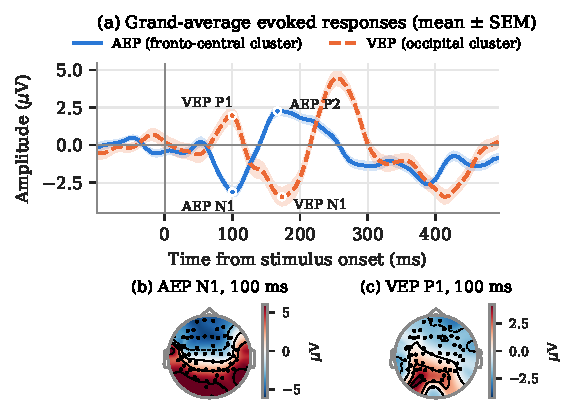
\includegraphics[width=\columnwidth]{fig_erp.pdf}
\caption{(a) Grand-average AEP (fronto-central cluster) and VEP (occipital cluster) after causal 1--30\,Hz filtering and CAR. (b, c) Scalp topographies at the AEP N1 and VEP P1 peaks.}
\label{fig:erp}
\end{figure}



\subsection{Single-Trial Discrimination}
Table~\ref{tab:cls} summarises the cross-validated performance. xDAWN-LDA identified the stimulated modality from single trials with \AccModX$\pm$\SdModX\,\% accuracy (AUC \AucModX; $p=\PermThousandP$, highest of 1000 permuted accuracies \PermNullMax\,\%). The Riemannian classifier performed equivalently on every task (e.g.\ \RieMod\,\% and \RieFour\,\%; all corrected $p\ge\RiePFour$). xDAWN-LDA was significantly better than Cluster-LDA ($p\le\PClusterMax$) and template matching on all tasks. On the 4-class problem it reached \AccFourX\,\% (chance \ChanceFour\,\%). Visual hemifield laterality was decoded with \AccVisLatX\,\% accuracy, whereas auditory ear laterality reached only \AccAudLatX\,\% (chance \ChanceAudLat\,\%; AUC \AucAudLatX). This asymmetry is expected: monaural tones reach both hemispheres, whereas hemifield checkerboards drive the contralateral occipital cortex. Accordingly, \AudConfShare\,\% of the 4-class errors were confusions between the left and right auditory stimuli, whereas modality was almost never confused. In the chronological calibrate-then-test split, accuracy was \ChronoMod\,\% (modality) and \ChronoFour\,\% (4-class).


\begin{table}[t]
\centering
\caption{Single-trial accuracy (\%, 10$\times$5-fold CV; mean $\pm$ SD over repetitions). $^{*}p<0.05$, $^{**}p<0.01$: worse than xDAWN-LDA (corrected resampled $t$-test).}
\label{tab:cls}
\setlength{\tabcolsep}{1.6pt}
\footnotesize
\begin{tabular}{lccccc}
\toprule
Task & Chance & xDAWN-LDA & Riem.-TS & Clust.-LDA & Templ. \\
\midrule
AEP vs.\ VEP & 50.3 & \textbf{98.2$\pm$0.2} & 97.8$\pm$0.5 & 92.2$\pm$1.2$^{**}$ & 80.1$\pm$1.1$^{**}$ \\
4-class & 25.3 & \textbf{83.9$\pm$2.0} & 81.0$\pm$1.1 & 71.2$\pm$1.4$^{**}$ & 53.7$\pm$1.5$^{**}$ \\
Aud.\ L vs.\ R & 50.3 & \textbf{71.2$\pm$2.8} & 67.0$\pm$2.1 & 58.6$\pm$2.5$^{*}$ & 53.0$\pm$3.3$^{**}$ \\
Vis.\ L vs.\ R & 51.0 & 97.6$\pm$0.6 & \textbf{97.8$\pm$0.2} & 93.2$\pm$1.3$^{*}$ & 75.8$\pm$3.8$^{**}$ \\
\bottomrule
\end{tabular}
\end{table}


Per class, both visual classes were recognised almost perfectly (recall \RecallLV\,\% and \RecallRV\,\%). The auditory classes reached \RecallLA\,\% and \RecallRA\,\%, and nearly all of their errors fell on the other ear. Cross-modal errors were rare (1.4\,\% of trials). A controller can thus trust the modality decision and treat the ear decision as a soft cue.



\subsection{Calibration Size and Averaging}\label{sec:avg}
Fig.~\ref{fig:det}(b) shows that modality accuracy rose from \LCfirst\,\% with \LCfirstN{} calibration trials to \LClast\,\% with \LClastN, so a short calibration block is sufficient. Averaging a few test trials of the same stimulus type before classification raised modality accuracy further, to \KavgAccB\,\% for $k=\KavgKB$ and \KavgAccC\,\% for $k=\KavgKC$. This setting assumes that repetitions of one stimulus can be grouped, as in a clinical test where the delivered stimulus is known and the question is whether the expected pathway responded. The classical peak criterion behaved very differently (Fig.~\ref{fig:det}(a)). The AEP N1 was found in \FairNSixteen\,\% of 16-trial and \FairNThirtyTwo\,\% of 32-trial averages, with false alarms at or below \FairNFa\,\%. The VEP P1, which is small (\VPamp\,$\mu$V) after hemifield stimulation and common-average referencing, reached only \FairPThirtyTwo\,\% detection at $k=32$ against \FairPFa\,\% false alarms. A threshold on a few electrodes thus needs tens of averages even for a large component and fails for a small one.

\begin{figure}[t]
\centering
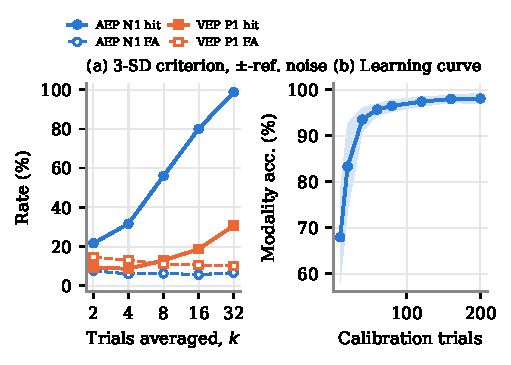
\includegraphics[width=\columnwidth]{fig_det.pdf}
\caption{(a) Hit rate (solid) and false-alarm rate (dashed) of the 3-SD peak criterion, with noise estimated from the $\pm$-reference, versus the number of averaged trials. (b) Modality accuracy of xDAWN-LDA versus the number of calibration trials (mean $\pm$ SD).}
\label{fig:det}
\end{figure}

\subsection{Control Analyses}\label{sec:ctl}
Table~\ref{tab:ctl} shows that neither the stimulus order nor the eyes explain the result. Although the previous stimulus predicts the current modality in \PrevPred\,\% of trials, decoding from the pre-stimulus windows or from 0--50\,ms stayed at chance (modality \PreMin--\PreMax\,\%, 4-class \PreFourMin--\PreFourMax\,\%). The \OffCycleN{} off-cycle trials were classified as accurately as the rest (modality \OffCycleMod\,\%). The EOG channel alone carried little information (visual laterality \EogVis\,\%, near chance; modality \EogMod\,\%). Regressing it out of the EEG (\EogRegMod\,\% and \EogRegVis\,\%) or removing the \FrontN{} frontal electrodes (\FrontMod\,\% and \FrontVis\,\%) left accuracy unchanged. The highest pre-stimulus 4-class value (\PreFourMax\,\%) is within the range expected by chance (binomial $p=0.08$ against 25.3\,\%), and the off-cycle trials also reached \OffCycleFour\,\% in the 4-class task ($n=\OffCycleN$, $p<10^{-4}$). The classifier therefore relies on post-stimulus cortical responses, not on the preceding stimulus, ocular activity or frontal electrodes.

\begin{table}[t]
\centering
\caption{Control analyses (xDAWN-LDA, 10$\times$5-fold CV accuracy in \%). Off-cycle: the 16 trials that did not follow the fixed stimulus cycle.}
\label{tab:ctl}
\setlength{\tabcolsep}{3pt}
\footnotesize
\begin{tabular}{lcccc}
\toprule
Input & AEP/VEP & off-cycle & 4-class & Vis.\ L/R \\
\midrule
Chance & 50.3 & & 25.3 & 51.0 \\
\midrule
Pre-stimulus $-200$--$0$\,ms & 50.2 & 41.2 & 29.3 & -- \\
Pre-stimulus $-100$--$0$\,ms & 50.6 & 53.1 & 25.1 & -- \\
Early $0$--$50$\,ms & 50.8 & 46.9 & 27.2 & -- \\
Standard $-100$--$500$\,ms & 98.2 & 99.4 & 83.9 & 97.6 \\
EOG channel only & 59.7 & -- & 31.4 & 54.5 \\
EEG, EOG regressed out & 98.3 & -- & 84.5 & 97.8 \\
EEG, 20 frontal ch.\ removed & 97.6 & -- & 83.8 & 97.6 \\
\bottomrule
\end{tabular}
\end{table}


\subsection{Real-Time Performance under ROS~2}
Table~\ref{tab:ros} reports the timing results. In every configuration each marker produced exactly one decision (\RosNdec/\RosNmark), and the streamed predictions matched the offline predictions on the held-out trials in \RosAgree\,\% of cases. With 20\,ms chunks at real-time speed, the mean excess latency was \RosExcess$\pm$\RosExcessSd\,ms (95th percentile \RosExcessP\,ms), and the mean marker-to-decision time was \RosTotal\,ms, of which 500\,ms is the epoch window itself. The excess grew with chunk length (\RosExTen\,ms for 10\,ms, \RosExForty\,ms for 40\,ms chunks), because the detector waits for the chunk holding the last epoch sample. The remainder is mainly the classifier, which took \RosProc\,ms at real-time speed. Under accelerated playback ($\times$5, $\times$10) the excess fell to \RosFastExMin--\RosFastExMax\,ms and the classification time to \RosFastProc\,ms, consistent with a higher CPU clock under sustained load; a performance governor would therefore reduce real-time latency further. At real-time speed the four nodes together used \RosCpuAll\,\% of one core and about \RosRss\,MB of memory, mostly Python overhead. The amplifier-emulating streamer was the most expensive node (\CpuStreamer\,\%); the detector used only \CpuDet\,\%.



\begin{table}[t]
\centering
\caption{End-to-end timing of the ROS 2 pipeline (all nodes on one host). Excess latency is measured from acquisition of the last epoch sample to the published decision.}
\label{tab:ros}
\setlength{\tabcolsep}{2.5pt}
\footnotesize
\begin{tabular}{lccccccc}
\toprule
Task & Chunk & Speed & Dec./Mark. & Excess (ms) & p95 & Classif. & Agree \\
 & (ms) & & & mean$\pm$SD & (ms) & (ms) & (\%) \\
\midrule
2-class & 10 & $\times$1 & 288/288 & 11.6$\pm$3.9 & 15.8 & 6.30 & 100 \\
2-class & 20 & $\times$1 & 288/288 & 15.4$\pm$5.6 & 22.5 & 6.50 & 100 \\
2-class & 40 & $\times$1 & 288/288 & 23.5$\pm$12.1 & 42.4 & 4.62 & 100 \\
4-class & 20 & $\times$1 & 288/288 & 10.0$\pm$5.9 & 17.6 & 2.25 & 100 \\
2-class & 20 & $\times$5 & 288/288 & 4.3$\pm$2.2 & 7.9 & 1.93 & 100 \\
2-class & 20 & $\times$10 & 288/288 & 3.8$\pm$5.3 & 6.2 & 1.70 & 100 \\
\bottomrule
\end{tabular}
\end{table}



\subsection{Middleware Overhead and Message Loss}
In a back-to-back real-time comparison, the excess latency was \RrExcess$\pm$\RrExcessSd\,ms with the four-node ROS~2 graph and \SpExcess$\pm$\SpExcessSd\,ms in a single process. Serialisation and two DDS hops therefore cost only \Overhead\,ms on average; chunk buffering and the classifier (\SpProc\,ms) dominate in both cases. The single-process run also reproduced the offline predictions exactly. Under fault injection (Table~\ref{tab:loss}), the detector recognised every gap from \texttt{data\_offset} and discarded the affected epochs. Survival followed the expected $(1-p)^{31}$ law, and every surviving held-out decision was identical to the offline one, so lost messages reduce throughput but never produce misaligned, wrong decisions. On lossy links, reliable QoS (used in all other runs) or short-gap interpolation is therefore advisable.

\begin{table}[t]
\centering
\caption{Fault injection: filtered chunks dropped at random ($\times$5 playback). Expected survival assumes an epoch is lost if any of its 31 chunks is lost. Agreement: surviving held-out decisions identical to offline.}
\label{tab:loss}
\setlength{\tabcolsep}{3pt}
\footnotesize
\begin{tabular}{lccccc}
\toprule
Drop rate & Gaps & Decisions & Survival & Expected & Agreement \\
\midrule
0.5\,\% & 72 & 249/288 & 86.5\,\% & 85.6\,\% & 100\,\% (130) \\
1.0\,\% & 139 & 219/288 & 76.0\,\% & 73.2\,\% & 100\,\% (114) \\
2.0\,\% & 275 & 159/288 & 55.2\,\% & 53.5\,\% & 100\,\% (87) \\
5.0\,\% & 686 & 52/288 & 18.1\,\% & 20.4\,\% & 100\,\% (33) \\
\bottomrule
\end{tabular}
\end{table}


\subsection{Robot Demonstration}
In the closed demonstration (Fig.~\ref{fig:robot}), the 4-class model drove turtlesim in real time for all \RobotN{} stimuli. On the \RobotHeldN{} held-out trials the executed action matched the intended one in \RobotAcc\,\% of cases (\RobotErr{} errors), because the ear confusions that limit 4-class accuracy map to the same action. Each command was published \RobotCmd\,ms (95th percentile \RobotCmdP\,ms) after the decision, or \RobotOnset$\pm$\RobotOnsetSd\,ms after stimulus onset (maximum \RobotOnsetMax\,ms).

\begin{figure}[t]
\centering
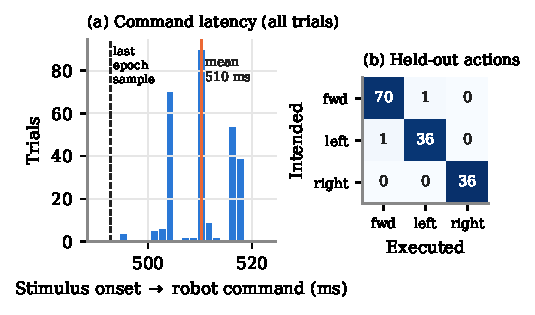
\includegraphics[width=\columnwidth]{fig_robot.pdf}
\caption{Closed robot demonstration. (a) Distribution of the time from stimulus onset to the turtlesim command; the dashed line marks the acquisition of the last epoch sample (\LastSample\,ms). (b) Intended vs.\ executed actions on the held-out half (counts).}
\label{fig:robot}
\end{figure}

\section{Discussion}
Carrying the filter state across chunks made streamed and offline signals identical, so an offline-calibrated model deploys without correction, and absolute sample indexing (\texttt{data\_offset}) protects epoch alignment against lost messages.

xDAWN-LDA and the Riemannian classifier performed equivalently, and xDAWN-LDA clearly outperformed the fixed-cluster and template baselines, most of all on the 4-class and auditory-laterality problems, where the discriminative information is spatially distributed. We deploy xDAWN-LDA because at run time it needs only a matrix and a dot product. Auditory laterality remained the hardest problem, in line with the bilateral representation of monaural sounds. Compared with the classical 3-SD criterion, which needs tens of averages and fails for small components, a short calibration block (about 40 trials for ${>}90$\,\% accuracy) is a modest price for single-trial decoding.

\paragraph*{Limitations} The evaluation uses a single subject and a single session from a public recording, so the accuracies should be read as a proof of concept rather than as population estimates. Multi-subject datasets such as ERP CORE~\cite{kappenman2021erpcore} are a natural next step. The stimuli followed a near-fixed order. Our controls argue strongly against a sequence effect, but a randomised design would remove the question entirely. The amplifier was emulated by file replay; a hardware driver will add its own buffering latency. The robot demonstration logs command publication, not physical actuation. Distributed (Wi-Fi) and embedded (\texttt{rclcpp}) deployment remain to be characterised, and no LSL comparison was made.

\section{Conclusion}
We presented an open ROS~2 pipeline that streams EEG, applies causal preprocessing and discriminates VEPs and AEPs trial by trial with xDAWN spatial filtering and shrinkage LDA. On public data it identified the stimulated modality in \AccModX\,\% of single trials and the exact stimulus class in \AccFourX\,\%, on par with a Riemannian classifier. Control analyses excluded the stimulus order and eye movements as explanations. Under ROS~2 it reproduced the offline decisions exactly, added only \RosExcess\,ms beyond the epoch window (\Overhead\,ms of it middleware), never misaligned epochs under message loss, and drove a simulated robot with \RobotAcc\,\% correct actions. The ROS~2 packages and the scripts that regenerate every figure and table are available at \url{https://github.com/vinothselvamani/vep-aep-ros2}. Future work will add hardware amplifier drivers, randomised multi-subject recordings and physical assistive devices.


\bibliographystyle{IEEEtran}
\bibliography{refs}

\end{document}
